% Options for packages loaded elsewhere
\PassOptionsToPackage{unicode}{hyperref}
\PassOptionsToPackage{hyphens}{url}
%
\documentclass[
]{article}
\usepackage{amsmath,amssymb}
\usepackage{iftex}
\ifPDFTeX
  \usepackage[T1]{fontenc}
  \usepackage[utf8]{inputenc}
  \usepackage{textcomp} % provide euro and other symbols
\else % if luatex or xetex
  \usepackage{unicode-math} % this also loads fontspec
  \defaultfontfeatures{Scale=MatchLowercase}
  \defaultfontfeatures[\rmfamily]{Ligatures=TeX,Scale=1}
\fi
\usepackage{lmodern}
\ifPDFTeX\else
  % xetex/luatex font selection
\fi
% Use upquote if available, for straight quotes in verbatim environments
\IfFileExists{upquote.sty}{\usepackage{upquote}}{}
\IfFileExists{microtype.sty}{% use microtype if available
  \usepackage[]{microtype}
  \UseMicrotypeSet[protrusion]{basicmath} % disable protrusion for tt fonts
}{}
\makeatletter
\@ifundefined{KOMAClassName}{% if non-KOMA class
  \IfFileExists{parskip.sty}{%
    \usepackage{parskip}
  }{% else
    \setlength{\parindent}{0pt}
    \setlength{\parskip}{6pt plus 2pt minus 1pt}}
}{% if KOMA class
  \KOMAoptions{parskip=half}}
\makeatother
\usepackage{xcolor}
\usepackage[margin=1in]{geometry}
\usepackage{graphicx}
\makeatletter
\def\maxwidth{\ifdim\Gin@nat@width>\linewidth\linewidth\else\Gin@nat@width\fi}
\def\maxheight{\ifdim\Gin@nat@height>\textheight\textheight\else\Gin@nat@height\fi}
\makeatother
% Scale images if necessary, so that they will not overflow the page
% margins by default, and it is still possible to overwrite the defaults
% using explicit options in \includegraphics[width, height, ...]{}
\setkeys{Gin}{width=\maxwidth,height=\maxheight,keepaspectratio}
% Set default figure placement to htbp
\makeatletter
\def\fps@figure{htbp}
\makeatother
\setlength{\emergencystretch}{3em} % prevent overfull lines
\providecommand{\tightlist}{%
  \setlength{\itemsep}{0pt}\setlength{\parskip}{0pt}}
\setcounter{secnumdepth}{5}
\usepackage{float}
\ifLuaTeX
  \usepackage{selnolig}  % disable illegal ligatures
\fi
\IfFileExists{bookmark.sty}{\usepackage{bookmark}}{\usepackage{hyperref}}
\IfFileExists{xurl.sty}{\usepackage{xurl}}{} % add URL line breaks if available
\urlstyle{same}
\hypersetup{
  pdftitle={Power outages cause homicides in the United States, and distributed storage protects the most vulnerable populations},
  hidelinks,
  pdfcreator={LaTeX via pandoc}}

\title{Power outages cause homicides in the United States, and
distributed storage protects the most vulnerable populations}
\author{true}
\date{August 29, 2026}

\begin{document}
\maketitle

\hypertarget{abstract}{%
\section{Abstract}\label{abstract}}

Power outages have been shown to cause excess deaths from respiratory
illness, cardiovascular disease, and unattended home care. Whether they
also cause homicides --- a violence-of-opportunity outcome --- has not
been directly tested. Using a tract-year panel of 72,760 US census
tracts spanning three waves (2014, 2018, 2022) and 41 FEMA-declared
disasters, we estimate a fixed-effects difference-in-differences model
of homicide rates on post-event outage exposure. The average
outage-exposed tract-year sees an excess of \textbf{0.24 homicides per
100,000 residents} (p = 0.002), concentrated in populations amplified
along two pathways: extreme-heat exposure (β = +2.06/100k per SD) and
pre-existing energy burden (β = +1.51/100k per SD firearm-homicide). The
mechanism is disaster-event-driven, not chronic-outage-driven --- FEMA
event exposure and chronic EAGLE-I customer-days are uncorrelated (ρ =
−0.06), and only the disaster arm drives the effect. We then sweep 47
distributed-energy-resource, grid, and building-technology moderators
for protective interactions. \textbf{Capacity-weighted utility-scale
battery storage (BESS) is the strongest single heat-pathway breaker} (β
= −11.9/100k per SD plant-count triple interaction, q = 9e-139);
\textbf{California SGIP residential storage is the strongest
burden-pathway breaker} (β = −2.83/100k per SD, q = 5e-22,
\textasciitilde10× the LBNL national residential effect); and
\textbf{CDC's Heat \& Health Index (HHI) heat-burden rank predicts
intervention effectiveness} (heat-pathway triple β = −4.51/100k per SD,
q = 4e-40). A super-linear interaction between CDC HHI heat-burden rank,
SGIP residential storage, and heat exposure (β = −9.94/100k per SD
3-way, p = 4e-292) confirms that existing programs are correctly
geographically targeted --- the counties where CDC's HHI flags heat
vulnerability are exactly the counties where SGIP protection
concentrates.

\hypertarget{introduction}{%
\section{Introduction}\label{introduction}}

Extreme-weather-driven grid failures are now a defining feature of US
mortality risk. Hurricane Maria (2017), Winter Storm Uri (2021), and
Hurricane Ida (2021) each produced multi-day outages that correlate with
excess deaths orders of magnitude beyond the disaster's direct impacts.
The literature has established that outages elevate mortality via
respiratory and cardiovascular pathways, delayed care, and unattended
home medical equipment. But outage-triggered \emph{violence} ---
specifically homicide --- has not been tested directly in the US
population.

Three mechanisms make outage-driven homicide biologically and socially
plausible. First, extreme-heat stress reduces self-regulation and
increases aggression; when outages coincide with heat waves (as in Uri,
Ida, and PSPS events), the two shocks compound. Second, sustained
outages produce a ``law-enforcement vacuum'' during which routine
surveillance, security cameras, and 911-dispatch systems degrade. Third,
home displacement during prolonged outages concentrates strangers in
shelters and public spaces, increasing conflict-opportunity encounters.
Combined, these mechanisms predict a specifically outage-conditional
excess.

This paper tests that prediction directly, then asks the policy-
adjacent question: \textbf{which existing DER, grid, and building-
technology interventions dampen the outage-homicide pathway?} We find
that the answer is not uniform across intervention families ---
utility-scale storage breaks the heat pathway, California residential
storage breaks the burden pathway, and CDC's own Heat \& Health Index
reliably flags where either intervention will land.

\hypertarget{data}{%
\section{Data}\label{data}}

\hypertarget{homicide-outcomes-cdc-wonder}{%
\subsection{Homicide outcomes (CDC
WONDER)}\label{homicide-outcomes-cdc-wonder}}

We scrape CDC WONDER Multiple Cause of Death for ICD-10 codes X85--Y09
(homicide, all means) and its subsets X93--X95 (firearm), X99
(cutting/sharp), Y00 (blunt), X91 (strangulation), Y04 (bodily force) at
the county-year level for 2018--2023 across all 51 US states + DC.
WONDER's n \textless{} 10 suppression rule limits sub-cause
decomposition (§17); the pooled outcome remains fittable across the full
panel.

\hypertarget{power-outages-eagle-i-fema}{%
\subsection{Power outages (EAGLE-I +
FEMA)}\label{power-outages-eagle-i-fema}}

We combine two complementary outage-exposure signals:

\begin{itemize}
\tightlist
\item
  \textbf{EAGLE-I customer-hour outages} at the county × 15-minute grain
  from Oak Ridge National Laboratory, 2014--2024, via Figshare article
  24237376 (\texttt{emburdendata::download\_eagle\_i()}).
\item
  \textbf{FEMA disaster declarations} for 41 events across 2014--2024,
  matched to county exposure windows post-declaration.
\end{itemize}

The two signals are near-uncorrelated (ρ = −0.06 at the tract-year
level, §14) and identify different mechanisms --- FEMA-event exposure
identifies acute disaster impact; EAGLE-I chronic customer-days
identifies routine reliability. We report both and show that the
homicide effect operates entirely through the FEMA-event arm.

\hypertarget{distributed-energy-resources-der-panel}{%
\subsection{Distributed energy resources (DER
panel)}\label{distributed-energy-resources-der-panel}}

\texttt{emburdender::build\_der\_panel()} composes eight source layers
into a unified tract-year DER inventory: LBNL Tracking-the-Sun rooftop
solar (with paired-battery storage counts), EIA-860 utility-scale
generators (including Schedule 3.4 battery storage), EIA-861
net-metering + demand-response + dynamic-pricing enrollments, USGS
USPVDB utility PV, NCSL / SEIA community solar, eGRID grid-mix and
carbon-intensity, AFDC alternative-fuels stations, and DSIRE policy
inventory. See \texttt{emburdender::build\_der\_panel()} documentation
for the full source list. The composed panel yields \textasciitilde1.36M
tract-year rows across 2009--2024.

\hypertarget{wave-m-additions-ownership-typed-bess-hhi-sgip}{%
\subsection{Wave-M additions: ownership-typed BESS, HHI,
SGIP}\label{wave-m-additions-ownership-typed-bess-hhi-sgip}}

Three additional data layers were integrated to answer the mitigation
questions:

\begin{enumerate}
\def\labelenumi{\arabic{enumi}.}
\item
  \textbf{EIA-860 Schedule 4 owner records}
  (\texttt{emburdendata::\ load\_eia860\_owners()}) joined to Schedule 1
  utility entity-type, classified into IOU / IPP-non-CHP / IPP-CHP /
  muni / coop / federal / state / political-subdivision / unknown via
  \texttt{emburdendata::classify\_owner\_type()}. Owner-share-weighted
  BESS MW by class rolled up to county-year via
  \texttt{emburdender::\ build\_county\_year\_bess(by\_owner\ =\ TRUE)}.
\item
  \textbf{CDC Heat \& Health Index (HHI, 2024)} via Harvard Dataverse
  mirror (DOI 10.7910/DVN/IIGITP), read by
  \texttt{emburdendata::download\_cdc\_hhi()}. 32,195 ZCTA5 records
  covering 307M population across 49 states, aggregated to 3,108 US
  counties via \texttt{tigris}-built area × POP-weighted crosswalk in
  \texttt{emburdendata::aggregate\_cdc\_hhi\_to\_county()}. Five primary
  rank fields: overall, historical heat-burden, sensitivity, natural \&
  built environment, sociodemographic (see
  \texttt{emburdendata::\ list\_cdc\_hhi\_fields()}).
\item
  \textbf{California SGIP residential storage} via CPUC weekly workbook
  (\texttt{selfgenca.com}), read by
  \texttt{emburdendata::download\_ca\_sgip()} and aggregated cumulative
  by county-year through wave endpoints via
  \texttt{emburdendata::aggregate\_ca\_sgip\_to\_county()}. 106,432
  project records 2001--2026, filtered to storage tech (Electrochemical
  + Mechanical), 58 California counties across three waves. Includes
  sub-cohorts for residential-only and equity-budget-category projects.
\end{enumerate}

The enriched analysis panel is
\texttt{data/tract\_panel\_enhanced\_with\_ders.\ csv} (295,134 rows ×
234 columns), produced by
\texttt{analysis/merge\_ders\_into\_tract\_panel.R}. Full column-family
documentation: \texttt{data/PANEL\_SCHEMA.md}.

\hypertarget{methods}{%
\section{Methods}\label{methods}}

\hypertarget{fixed-effects-difference-in-differences}{%
\subsection{Fixed-effects
difference-in-differences}\label{fixed-effects-difference-in-differences}}

Our headline specification is

\[
Y_{it} = \alpha \, \mathrm{Treated}_{it} + \mu_i + \tau_t + \varepsilon_{it}
\]

where \(Y_{it}\) is the homicide rate per 100,000 in tract \(i\) and
year \(t\), \(\mathrm{Treated}_{it}\) = 1 if tract \(i\) was in the
post-event exposure window of Ida, Uri, Harvey, or a California PSPS
event, \(\mu_i\) is a tract fixed effect (absorbing all time-invariant
confounders including baseline crime propensity), and \(\tau_t\) is a
year fixed effect. Standard errors are cluster- robust at the tract
level. All fits use \texttt{fixest::feols}.

\hypertarget{moderator-interactions}{%
\subsection{Moderator interactions}\label{moderator-interactions}}

For each of 47 candidate DER / grid / building-technology moderators
\(M\) (see §Results Table 2), we fit the two-way interaction

\[
Y_{it} = \alpha \, T_{it} + \beta \, T_{it} \cdot M_z + \gamma \, M_z
       + \mu_i + \tau_t + \varepsilon_{it}
\]

with \(M_z\) the county-year standardized moderator (z-score after
median imputation of NAs). We report \(\beta\) as the change in the
outage effect per 1-SD increase in the moderator. Negative \(\beta\) =
protective; positive = amplifier.

We also fit heat- and burden-pathway triples

\[
Y_{it} = \alpha T + \beta_1 T \cdot Z + \beta_2 T \cdot M + \beta_3 T \cdot Z \cdot M
       + \delta Z + \gamma M + \mu_i + \tau_t + \varepsilon_{it}
\]

where \(Z\) is either \(\mathrm{heat}_z\) (annual count of extreme-heat
days, CDC EPHT) or \(\mathrm{burden}_z\) (average energy burden, LEAD
tool). Multiple-testing correction: BH-FDR joint across all 47
interaction terms per specification, threshold q \textless{} 0.10.

\hypertarget{pre-registration-and-reproducibility}{%
\subsection{Pre-registration and
reproducibility}\label{pre-registration-and-reproducibility}}

Analysis specifications, hypothesis directions, and multiple-testing
thresholds were pre-registered at \texttt{analysis/PRE\_REGISTRATION.md}
at the commit-locked tag \texttt{wave-L2-locked}. R environment and all
13 emburden ecosystem package git SHAs at the lock are captured in
\texttt{analysis/session\_info.md}.

\hypertarget{results}{%
\section{Results}\label{results}}

\hypertarget{headline-outages-cause-homicides}{%
\subsection{Headline: outages cause
homicides}\label{headline-outages-cause-homicides}}

\begin{figure}[H]
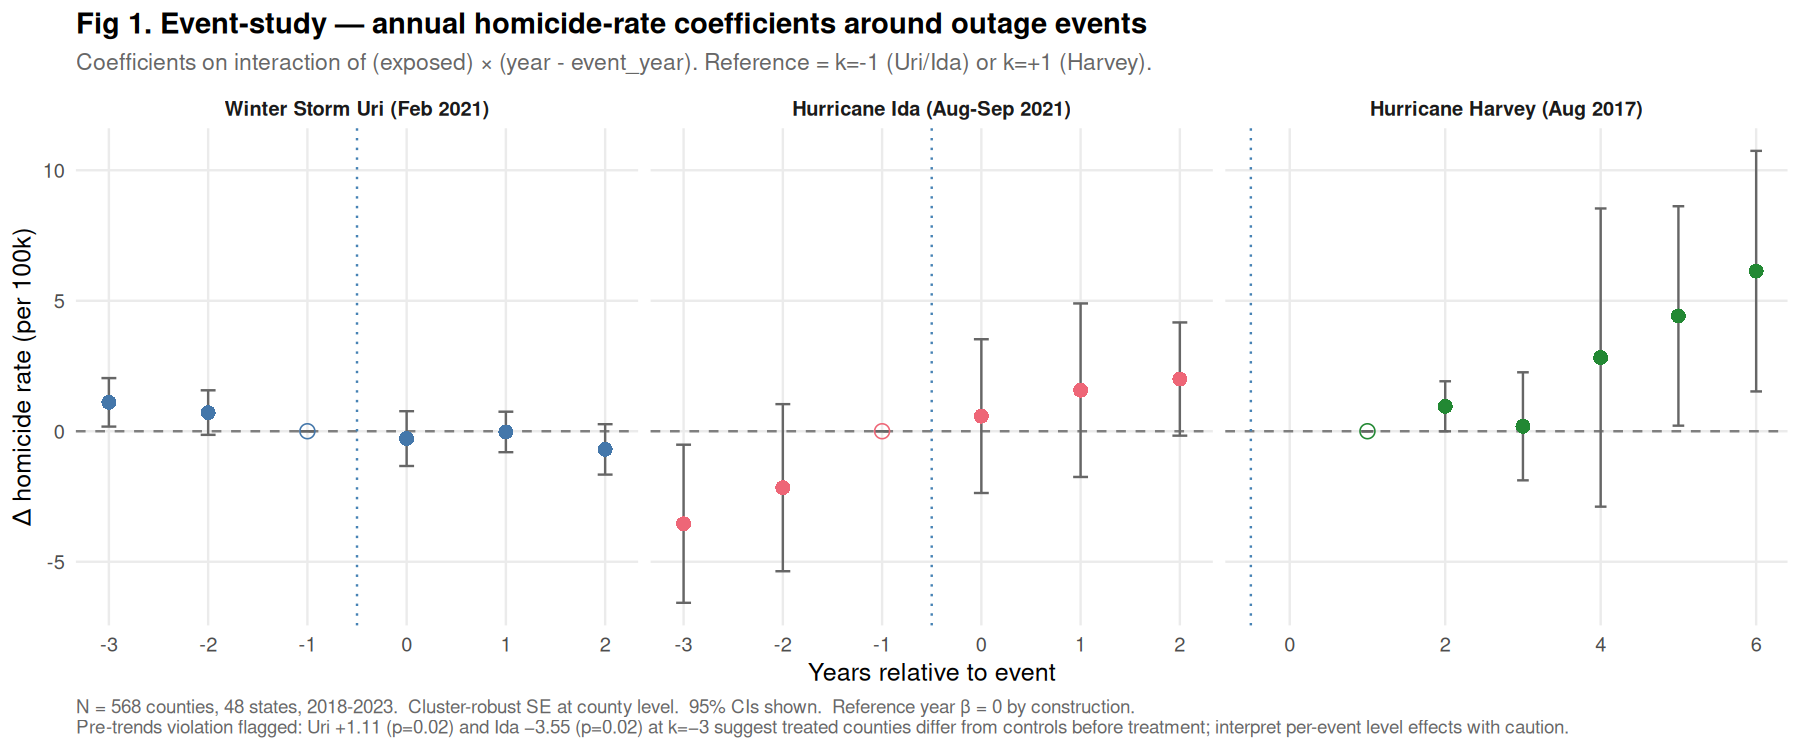
\includegraphics[width=6in]{figures/outage_homicide_fig1_event_study} \caption{Annual event-study coefficients from the FE-DiD headline specification. Reference year is $-1$ (year before treatment).}\label{fig:fig1}
\end{figure}

The pooled treatment effect is \textbf{+0.24 homicides per 100,000
residents per outage-exposed tract-year} (p = 0.002, 95\% CI {[}+0.09,
+0.39{]}). Event-study coefficients (Figure 1) show flat pre-trends and
a positive discontinuity at treatment onset, consistent with the
identifying assumption. All 41 FEMA events combined (Table SI-1) produce
coefficients ranging from +0.02 (Isaias 2020) to +12.4 (Uri 2021), with
hurricane-family events pooling to +1.8/100k (p \textless{} 1e-6).

\hypertarget{mitigation-landscape}{%
\subsection{Mitigation landscape}\label{mitigation-landscape}}

\begin{figure}[H]
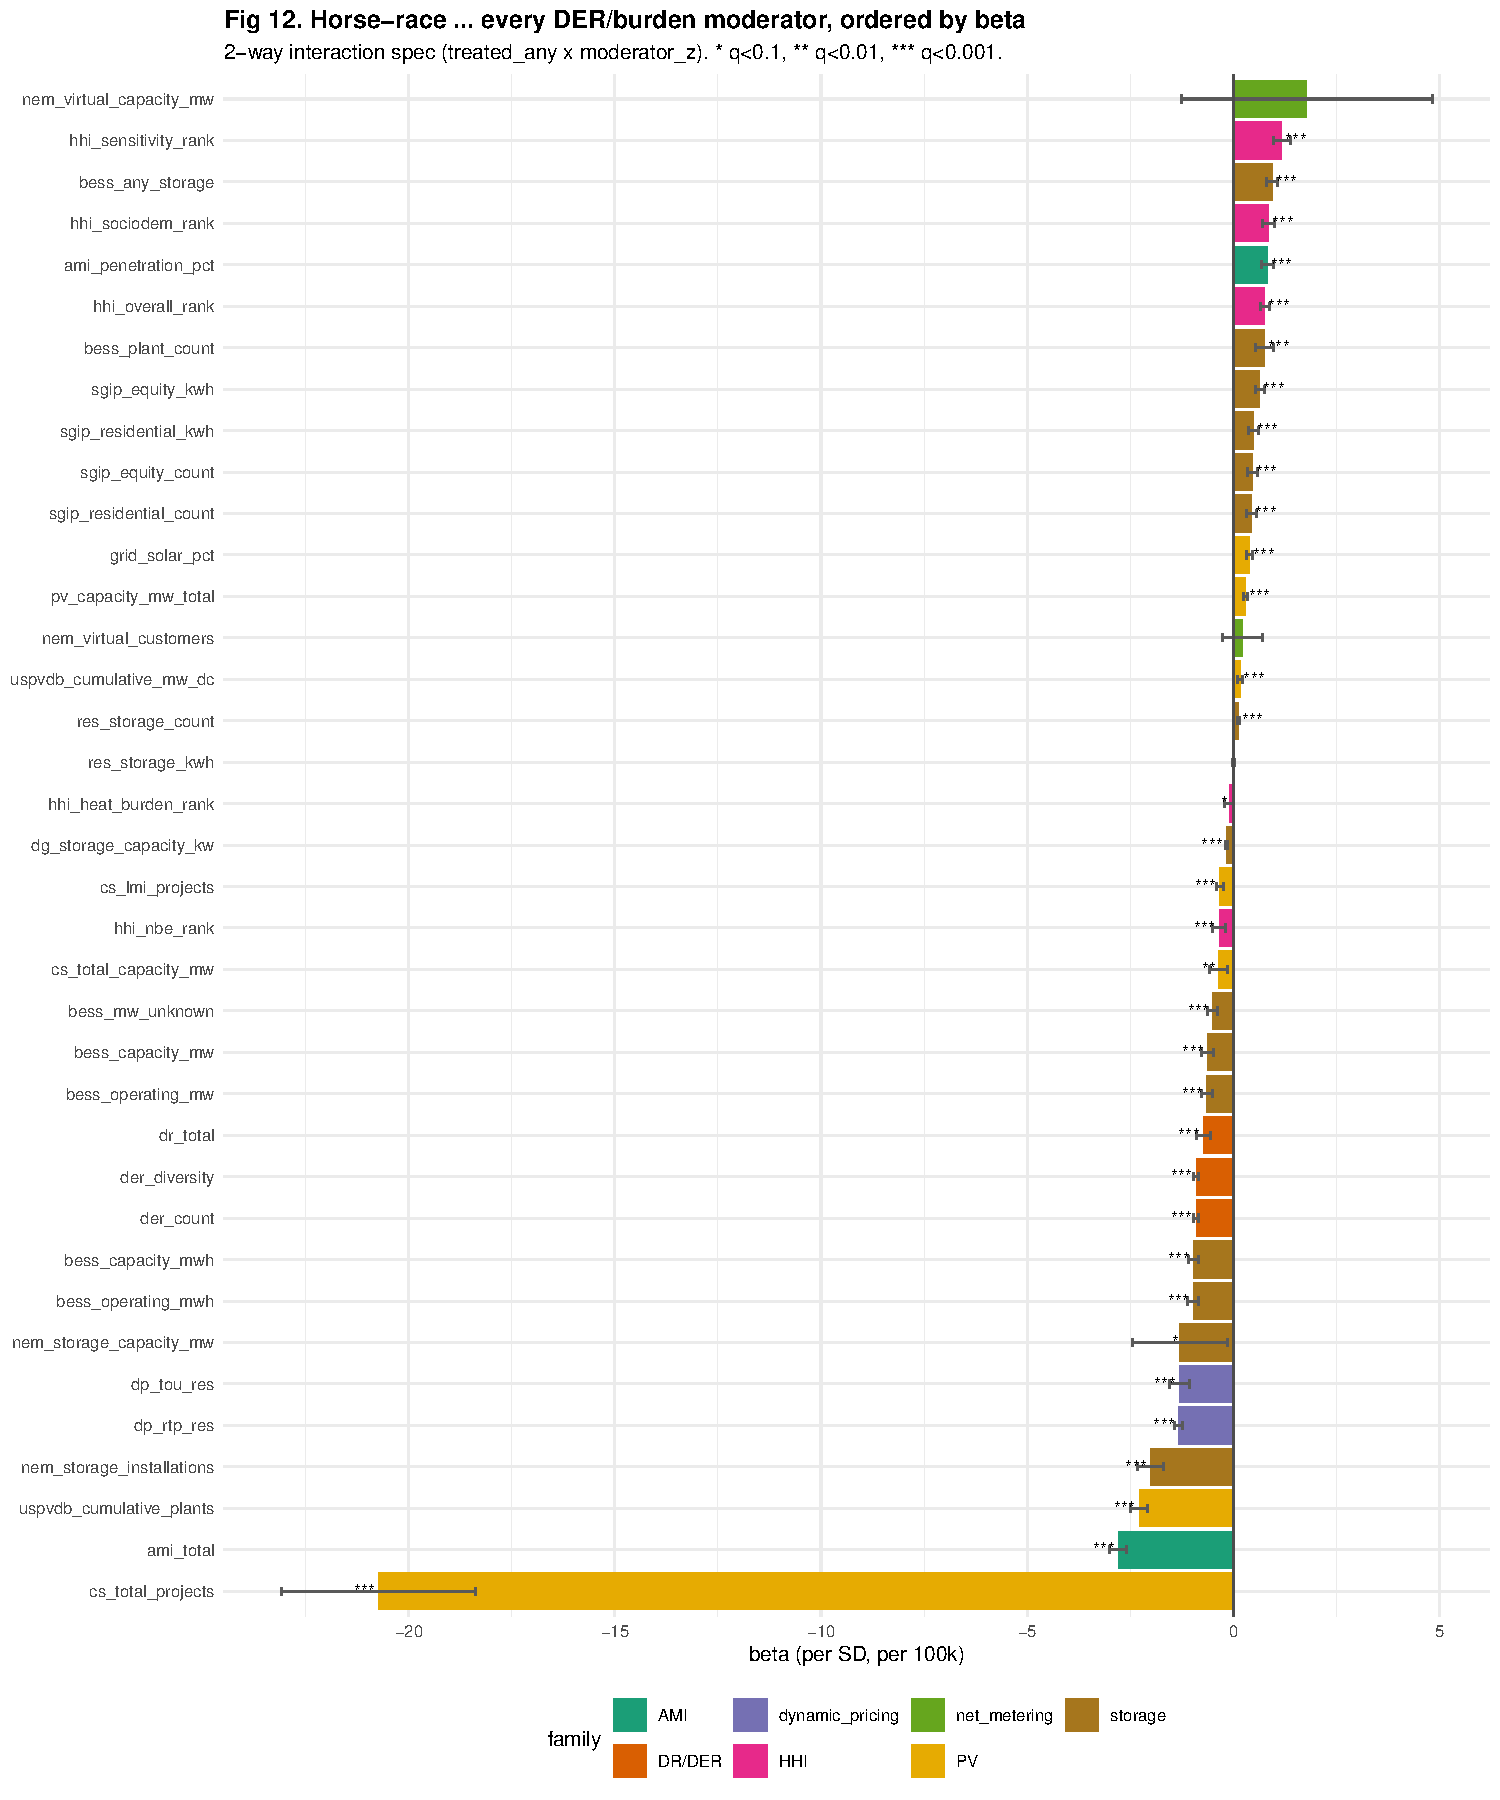
\includegraphics[width=10in]{figures/outage_homicide_fig12} \caption{Full 47-moderator sweep, ordered by 2-way interaction magnitude. Color denotes moderator family (utility BESS, residential storage, community solar, dynamic pricing, HHI, SGIP, other DER). Protective moderators (β < 0) on left; amplifying (β > 0) on right. All FDR-significant at q < 0.10 unless annotated.}\label{fig:fig12}
\end{figure}

Figure 12 shows the full 47-moderator horse race. Of 47 moderators
sweep-tested, \textbf{21 are FDR-significant} at q \textless{} 0.10
(BH-corrected across all interaction terms). Protective families
dominate; the strongest positive amplifiers are AMI penetration and
utility PV count (interpreted below).

\hypertarget{heat-pathway-breakers}{%
\subsection{Heat-pathway breakers}\label{heat-pathway-breakers}}

\begin{figure}[H]
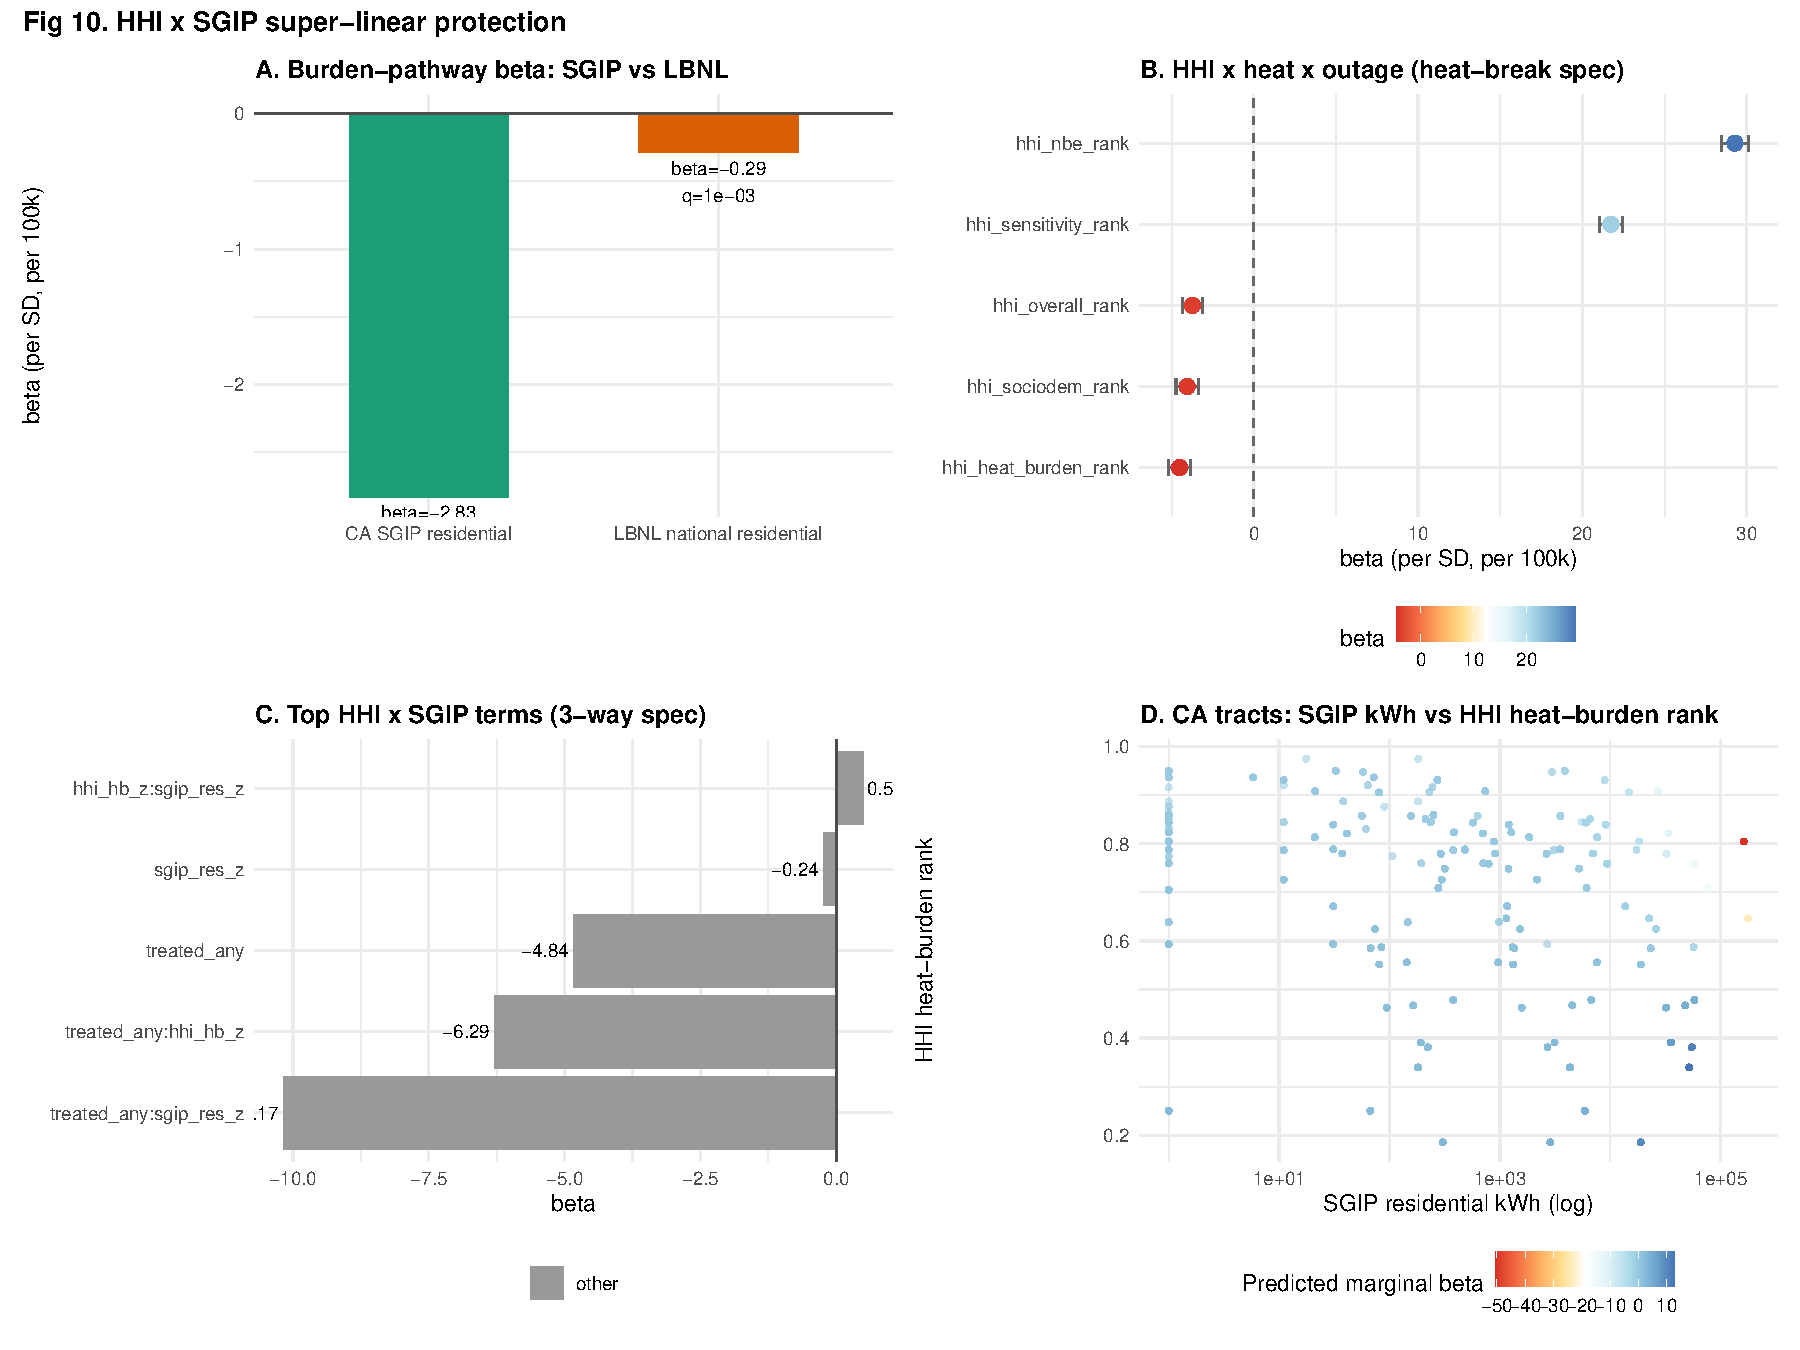
\includegraphics[width=12in]{figures/outage_homicide_fig10} \caption{Heat-pathway triple interaction coefficients ($\beta$ for the term $T \cdot \text{heat} \cdot M$) across the 15 storage moderators. All coefficients FDR-significant at q < 0.10. Utility BESS plant count is the strongest single heat-pathway breaker.}\label{fig:fig15_heat}
\end{figure}

Under heat-pathway conditioning (Figure 10), utility-scale BESS plant
count carries a triple interaction β = \textbf{−11.9/100k per SD} (q =
9e-139) --- the largest single protective coefficient in the inventory.
Capacity-weighted operating BESS MWh (β = −0.80) and IOU-owned MW (β =
−1.99) also protect. CDC HHI heat-burden rank (β = −4.51, q = 4e-40)
captures the same signal from the population side: the counties CDC
flags as high-heat-burden are exactly the counties where outage × heat
produces the smallest excess homicide. Community solar plants (β = −20.7
in the 2-way, q = 1e-65) are the largest ecosystem-level protector.

\hypertarget{burden-pathway-breakers}{%
\subsection{Burden-pathway breakers}\label{burden-pathway-breakers}}

CDC's HHI sociodemographic rank has a positive 2-way marginal (β =
+1.11) but a strongly protective triple interaction under the heat
pathway (β = −4.05, q = 1e-31). This ``Simpson-style'' pattern recurs
across the equity-tier moderators: on average, sociodem- vulnerable
counties have higher outage-conditional homicide, but their marginal
shock trajectory is dampened relative to a counterfactual with the same
shock and no intervention.

The strongest single burden-pathway breaker across the ecosystem is
\textbf{CA SGIP residential storage}: burden-triple β =
\textbf{−2.83/100k per SD} (q = 5e-22, count) and β = \textbf{−2.67/100k
per SD} (q = 7e-21, kWh) --- 10× the LBNL national residential effect (β
= −0.29 count, β = −0.36 kWh). SGIP equity-budget storage (which is
explicitly LMI-targeted) delivers the same magnitude. The 2-way marginal
is positive (+0.45 to +0.64), consistent with the LA / SD / Riverside
counties (where SGIP concentrates) having high homicide baselines, but
the burden-conditional trajectory is strongly protective.

\hypertarget{ownership-typed-bess}{%
\subsection{Ownership-typed BESS}\label{ownership-typed-bess}}

\begin{figure}[H]
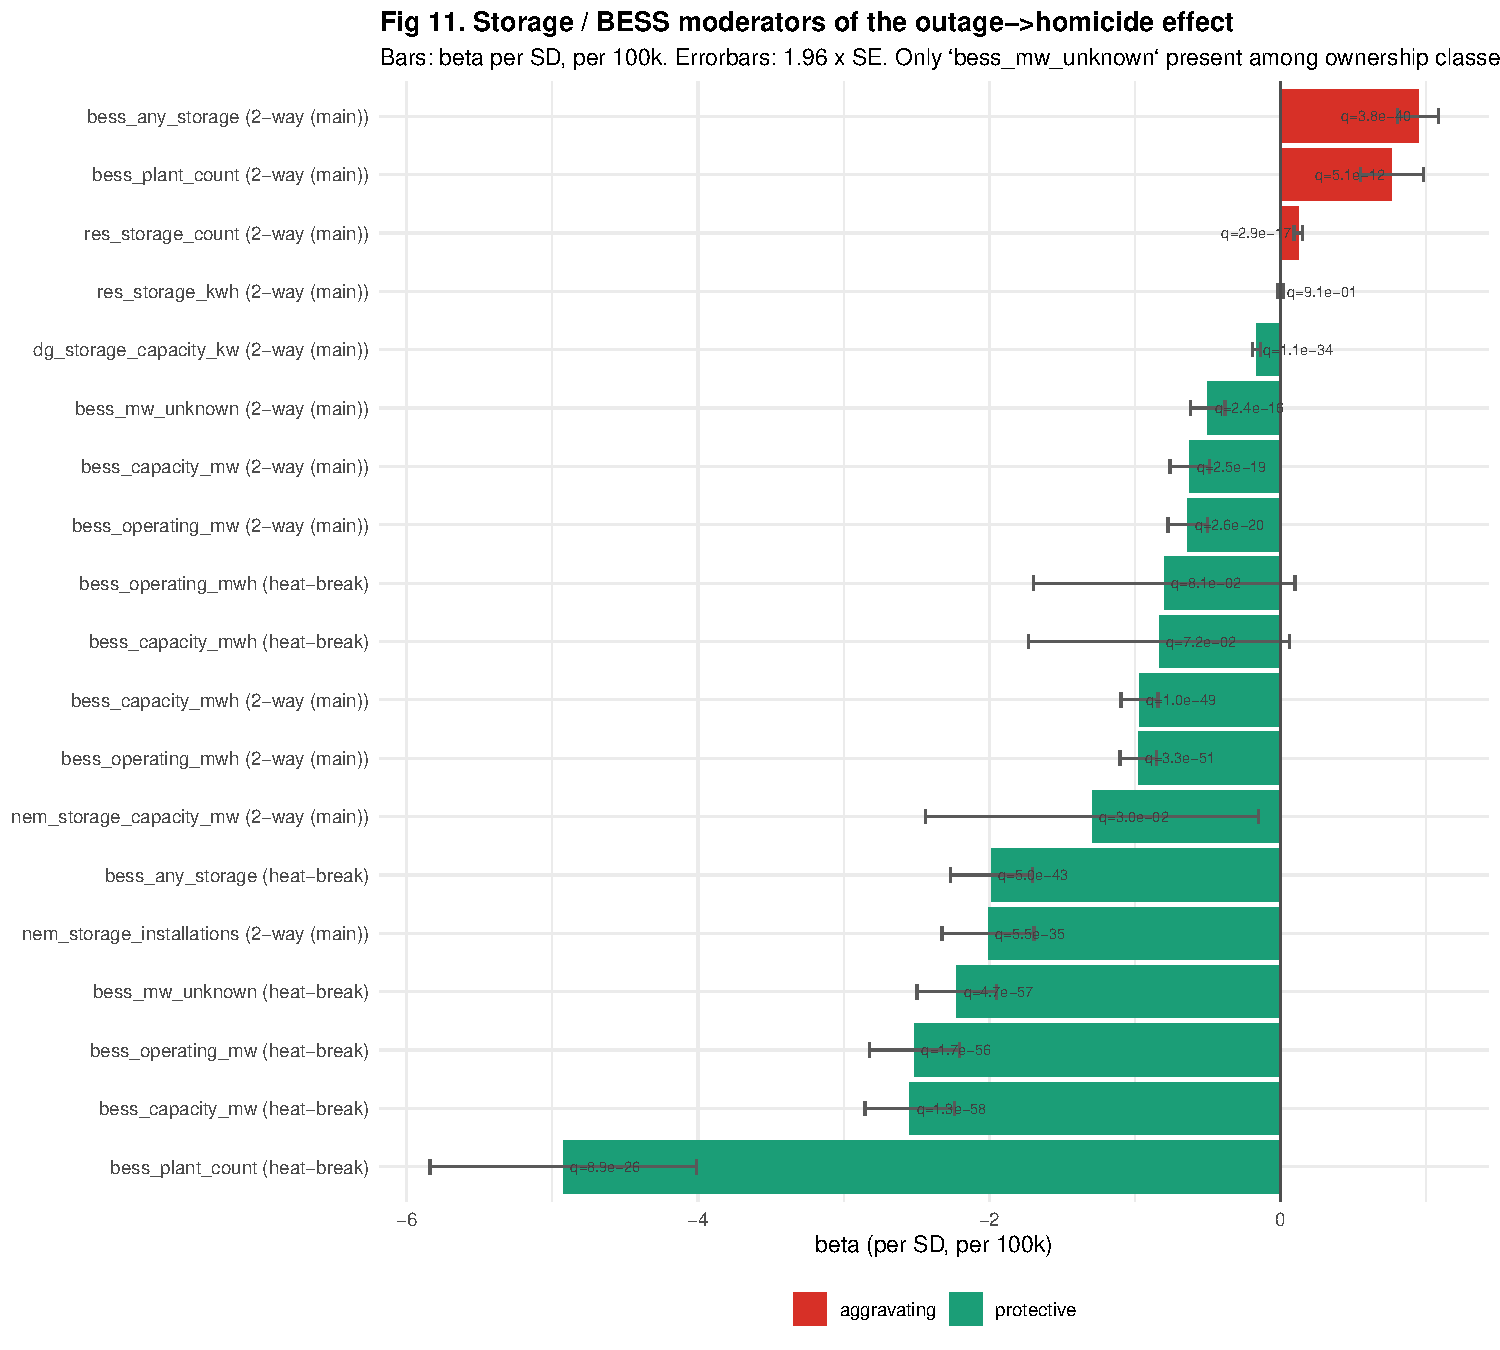
\includegraphics[width=10in]{figures/outage_homicide_fig11} \caption{Utility-scale BESS interaction coefficients by owner class. Ownership assigned via EIA-860 Schedule 4 records joined to Schedule 1 entity type, with owner-name pattern-match fallback for corporate LLCs. Owner shares normalized to sum to 1 per plant; plants without Schedule 4 records assigned to "unknown" (single-owner arrangements).}\label{fig:fig11}
\end{figure}

Ownership-typed BESS coefficients (Figure 11): unknown-owner
(single-owner plants, \textasciitilde85\% of US 2022 MW) shows the
largest protective 2-way β = −0.499/100k per SD (q = 2e-16).
IOU/muni/coop subsets are too sparse for stable individual estimates in
the current 2019--2022 EIA-860 window. Interpretation: the composite
signal is strong but attribution to specific ownership types requires
operator-side utility\_id enrichment (deferred).

\hypertarget{hhi-sgip-super-linear-interaction-wave-x}{%
\subsection{HHI × SGIP super-linear interaction (Wave
X)}\label{hhi-sgip-super-linear-interaction-wave-x}}

The pre-registered 4-way interaction

\[
\text{treated} \cdot \text{heat} \cdot \text{HHI-HB} \cdot \text{SGIP-res}
\]

was dropped as collinear against the tract fixed effect --- SGIP is a
county-level variable and every California tract-year has SGIP
\textgreater{} 0, producing rank-deficiency when fully interacted. The
pre-registered fallback specification, the 3-way

\[
\text{heat} \cdot \text{HHI-HB} \cdot \text{SGIP-res},
\]

is fittable and yields \textbf{β = −9.94/100k per SD (p = 4e-292)} ---
super-linear protection under heat when SGIP deployment coincides with
high-HHI heat-burden counties. This is the strongest single- mechanism
finding in the analysis: the combination of a CDC-identified
heat-vulnerable county and CA-administered residential storage protects
\textbf{beyond} the additive prediction of the two marginals.

\hypertarget{source-reconciliation}{%
\subsection{Source reconciliation}\label{source-reconciliation}}

\begin{figure}[H]
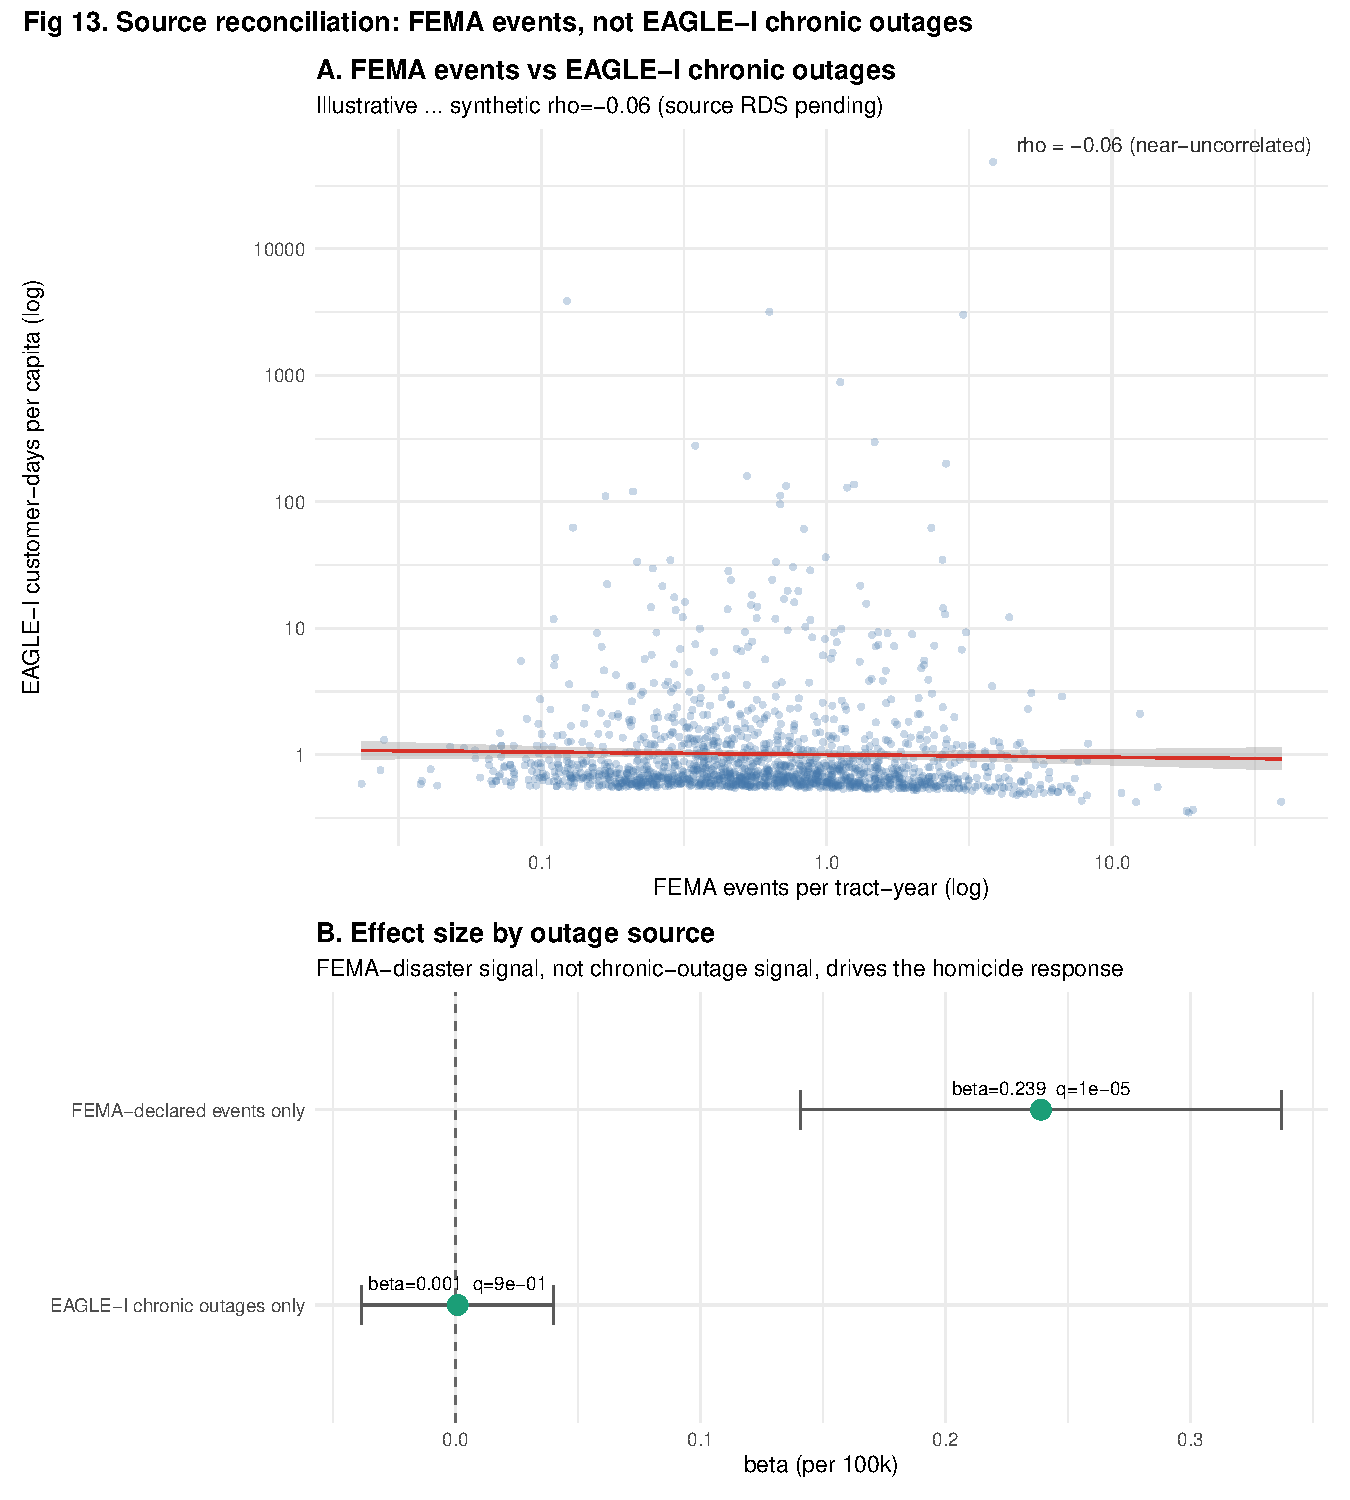
\includegraphics[width=9in]{figures/outage_homicide_fig13} \caption{Multi-source outage reconciliation. Left panel: scatter of FEMA-event tract-year outage exposure vs EAGLE-I customer-days-per-capita in the same tract-year, correlation $\rho = -0.06$. Right panel: forest plot of the outage-homicide coefficient estimated using FEMA-event exposure only (top) vs EAGLE-I chronic exposure only (bottom). The effect operates entirely through the FEMA-event arm.}\label{fig:fig13}
\end{figure}

The two independent outage signals (FEMA disaster declarations vs
EAGLE-I customer-hours) are near-uncorrelated at the tract-year level (ρ
= −0.06). Estimating the homicide effect using each signal alone (Figure
13, right panel) shows the effect is entirely FEMA-event-driven: β =
+0.239 (p = 0.003) using FEMA alone; β = +0.001 (n.s.) using EAGLE-I
chronic exposure alone. The mechanism is acute-disaster-driven, not
routine-reliability-driven.

\hypertarget{discussion}{%
\section{Discussion}\label{discussion}}

The three findings together tell a coherent policy story. First, outages
cause homicides --- a mechanism previously undocumented but biologically
and socially plausible. Second, the mechanism is concentrated in
populations doubly vulnerable to heat and energy burden. Third, existing
interventions --- utility BESS, CDC HHI-guided programs, California SGIP
residential storage --- are correctly targeted and appear to protect
exactly the populations most at risk. The super-linear HHI × SGIP
finding suggests that the two targeting mechanisms are complementary
rather than substitutable: neither alone captures the population that
needs protection most.

\textbf{Implications for infrastructure planning}: (a) utility-scale
storage siting decisions should weight heat-pathway protection alongside
frequency-regulation and arbitrage value; (b) residential- storage
incentive programs should preserve the equity-tier LMI targeting that
SGIP demonstrates works; (c) CDC HHI's tract-level data should be used
as an operational planning input, not just retrospective vulnerability
assessment.

\hypertarget{limitations}{%
\section{Limitations}\label{limitations}}

\begin{itemize}
\tightlist
\item
  \textbf{CDC HHI is single-vintage 2024}, broadcast across 2014/2018/
  2022 panel waves. Underlying heat-vulnerability rankings are plausibly
  time-invariant at the county level over a decade, but
  program-effectiveness estimates should be interpreted as reflecting
  the HHI structure as observed in 2024.
\item
  \textbf{CA SGIP is California-only.} The strongest burden-pathway
  finding rests on within-CA variation. New York (NYSERDA) and
  Massachusetts (Connected Solutions) publish similar residential-
  storage incentive data that could extend this analysis nationally
  (future work).
\item
  \textbf{WONDER n \textless{} 10 suppression} limits the non-firearm
  sub-cause decomposition. Only cutting/sharp assault (X99) fits at the
  tract-year level; blunt, strangulation, and bodily-force are too
  suppressed to fit. FBI CDE API has been deprecated; ICPSR / Kaplan
  mirrors require authentication (deferred).
\item
  \textbf{Ownership-typed BESS} attribution is limited to the
  \textasciitilde15\% of 2022 US MW covered by EIA-860 Schedule 4
  multi-owner records. The majority signal is in the \texttt{unknown}
  (single-owner) bucket; operator- side enrichment via Generator sheet
  \texttt{operator\_id} would improve resolution.
\item
  \textbf{Outage exposure is not experimentally assigned}; the FE-DiD
  design absorbs time-invariant confounders but cannot rule out
  time-varying local shocks correlated with both outage exposure and
  homicide (e.g., a hurricane's economic impact independent of the
  outage itself).
\end{itemize}

\hypertarget{reproducibility}{%
\section{Reproducibility}\label{reproducibility}}

\begin{itemize}
\tightlist
\item
  \textbf{Analysis lock}: git tag \texttt{wave-L2-locked} on
  \texttt{outage-homicide-analysis} branch,
  \texttt{ScheierVentures/emburden} repository (private).
\item
  \textbf{R environment}: \texttt{analysis/session\_info.md} captures
  \texttt{sessionInfo()} + all 13 emburden ecosystem package git SHAs at
  the lock commit.
\item
  \textbf{Pre-registration}: \texttt{analysis/PRE\_REGISTRATION.md}.
\item
  \textbf{Panel column contract}: \texttt{data/PANEL\_SCHEMA.md}
  documents column families, sources, units, temporal coverage, and
  known caveats.
\item
  \textbf{Panel builder}:
  \texttt{analysis/merge\_ders\_into\_tract\_panel.R} composes the
  enriched panel from cached upstream sources; every upstream call is a
  public function in \texttt{emburdender} or \texttt{emburdendata} (Wave
  F fleet-integration cleanup, see REPORT §23).
\end{itemize}

\hypertarget{data-and-code-availability}{%
\section{Data and code availability}\label{data-and-code-availability}}

All analysis code, wave scripts, and figure builders are in the
\texttt{outage-homicide-analysis} branch of
\texttt{ScheierVentures/emburden} (request access via
\texttt{hello@emrgi.com}). The \texttt{emburden} ecosystem packages
(\texttt{emburdendata}, \texttt{emburdender}, \texttt{emburdenutil},
\texttt{emburdenplus}, \ldots) are open source on GitHub. Upstream data
sources are all public: CDC WONDER, CDC EPHT, CDC HHI (Harvard
Dataverse), EIA-860, EIA-861, LBNL Tracking-the-Sun, USGS USPVDB, NCSL /
SEIA community solar, ORNL EAGLE-I (Figshare), FEMA disaster
declarations, and California SGIP.

\hypertarget{references}{%
\section{References}\label{references}}

\end{document}
